\section{RANSAC with Ellipse I (18)}

In this exercise, you are tasked to detect an ellipse based on given dataset using RANSAC.
\begin{figure}[H]
    \centering
    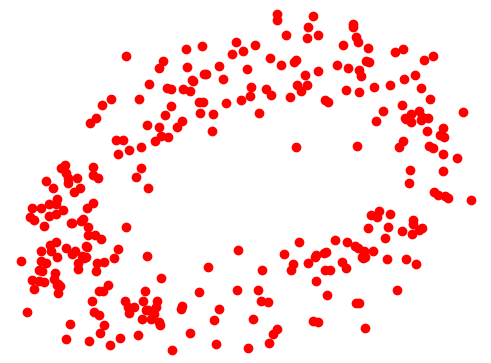
\includegraphics[width=0.65\textwidth]{img/ellipse.png}
    \caption{A Plot of Randomly Selected Dataset}
    \label{fig:p3c1}
\end{figure}
The goal is to estimate the parameters $\mathbf{Q}$ and $\mathbf{b}$ by fitting the sensor data to an ellipse. 
An ellipse can be described by the quadratic equation: 
\begin{equation*}
(\mathbf{p}-\mathbf{b})^\top\mathbf{Q}(\mathbf{p}-\mathbf{b})=1
\end{equation*}
or
\begin{equation*}
    Ax^2+2Bxy+Cy^2-2Dx-2Ey+1=0
\end{equation*}
where:
\begin{itemize}
\item $\mathbf{Q}=\mathbf{Q}^\top\in\mathbb{R}^{2\times2}$ is a unique symmetric positive definite matrix of coefficients. [If $\mathbf{Q}$ is not positive definite, you may have a hyperbola instead.]
\end{itemize}
Note that the coefficients ($A$,$B$,$C$,$D$,and $E$) are also unique.
The conversion from the polynomial coeffcients to the quadratic form can be expressed as follows:
\begin{equation*}
    \begin{aligned}
        \mathbf{Q}&=\alpha\begin{bmatrix}
        A & B\\ B & C
    \end{bmatrix}\\
    \mathbf{Q}\mathbf{b}&=\alpha\begin{bmatrix}
        D\\E
    \end{bmatrix}\\
    \alpha&=\frac{1}{\begin{bmatrix}
        D & E
    \end{bmatrix}\begin{bmatrix}
        A & B \\ B & C
    \end{bmatrix}^{-1}\begin{bmatrix}
        D \\ E
    \end{bmatrix}-1}
    \end{aligned}
\end{equation*}

\begin{enumerate}[a.)]  
\item Determine the minimum number of points to uniquely determined ellipse's parameters as well as derive a method to construct an ellipse with the parameters ($A$,$B$,$C$,$D$, and $E$) based on those points. $\mathbf{p}_i=(x_i,y_i)$ denote the $i^\text{th}$ data point. You must explain your rationale to receive credits. [10 pts]
\item 
Fit an ellipse with the following datasets and compute for $\mathbf{Q}$, $\mathbf{b}$, $A$, $B$, $C$, $D$ and $E$.

\begin{equation*}
    (2.92, -6.01), \quad (3.40, -7.20), \quad (4.99, -7.84), \quad (5.48, -7.04), \quad (4.20, -5.91)
\end{equation*}

 You don't have code for this part, but you still have to do it with Python in the next part. [8 pts.]
\end{enumerate}
